\section{\huge ROOMLanguage}
	Real Time Object Oriented Modeling (ROOM) is a language ... 
	
		\subsection{\huge LogicalModel}
		The LogicalModel describes the logical structure and behavior of a ROOM application. The LogicalModel an its elements can be mapped on any PhysicalModel and its elements...
	
		
		
		\subsubsection{\huge ActorClass}
			\hypertarget{ref:ActorClass}{}
			
			\textbf{Description:} The actor is the basic structural building block for building systems with ROOM. An actor can be refined hierarchically and thus can be of arbitrarily large scope. Ports define the interface of an actor. An actor can also have a behavior usually defined by a finite state machine. 
			
			
			\begingroup
			%\setlength{\tabcolsep}{10pt} % Default value: 6pt
			\renewcommand{\arraystretch}{1.8} % Default value: 1
			\begin{longtable}{p{2.5cm}|p{4cm} p{.5\textwidth}}
				\multicolumn{2}{l}{\textbf{\large Features}} & \\
				\hline
			\multirow{9}{*}{Contains:} & \tabitem \hyperlink{ref:ActorRef}{ActorRef}  & An ActorRef ...description\\
			& \tabitem \hyperlink{ref:Port}{Port}  & A Port is an instance of a ProtocolClass and the only interface for an ActorClass. It provides strong decoupling of ActorClasses from each other, thus enabling easy testability, reusability and deployment of Actors to different threads or nodes.description  \\
			& \tabitem \hyperlink{ref:SAP}{SAP}  & An SAP ....description  \\
			& \tabitem \hyperlink{ref:SPP}{SPP}  & An SPP ... description \\
			& \tabitem \hyperlink{ref:Binding}{Binding}  & A Binding connects two Ports with each otherdescription \\
			& \tabitem \hyperlink{ref:LayerConnection}{LayerConnection}  & A LayerConnection ... description  \\
			& \tabitem \hyperlink{ref:Attribute}{Attribute}  & An Attribute is a member variable of a class.  \\
			& \tabitem \hyperlink{ref:Operation}{Operation}  & An Operation is a member function of a class (ActorClass, ProtocolClass, DataClass, ...)description  \\
			& \tabitem \hyperlink{ref:StateMachine}{StateMachine}  & A StateMachine describes the state based, event driven behavior of an ActorClass \\
			\hline
			Uses: & \tabitem \hyperlink{ref:Inheritance}{Inheritance}  & Inheritance bla\\
			\hline
			\end{longtable}
			\endgroup
			
			\begingroup
			%\setlength{\tabcolsep}{10pt} % Default value: 6pt
			\renewcommand{\arraystretch}{1.8} % Default value: 1
			\begin{longtable}{p{2.5cm}|p{4cm} p{.5\textwidth}}
				\multicolumn{2}{l}{\textbf{\large Related Features}} & \\
				\hline
			Typecasts: & \tabitem \hyperlink{ref:ActorRef}{ActorRef}  & An ActorRef ...description\\
			\hline
			Is contained in: & \tabitem \hyperlink{ref:LogicalModel}{LogicalModel}  & The LogicalModel describes the logical structure and behavior of a ROOM application. The LogicalModel an its elements can be mapped on any PhysicalModel and its elements...\\
			\hline
			Is edited by: & \tabitem \hyperlink{ref:GraphicalStructureEditor}{GraphicalStructureEditor}  & The Structure Editor allows to edit the Actor Structure in a convenient way. It is possible to create and arrange actor references and ports and to create bindings and layer connections.\\
			\hline
			\end{longtable}
			\endgroup
			
			some more about ActorClass, graphical and textual notation, concepts, ...
			
			\textbf{Example:} 
				\textbf{Graphical Notation}
				\\
					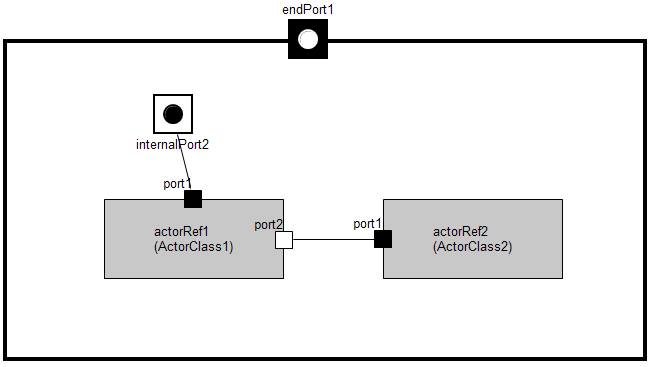
\includegraphics[width=\textwidth]{images/300-SimpleActorClassStructure.png}
				\\
				\textbf{Textual Notation}
				\\
					\begin{lstlisting}[language=ROOM]
					ActorClass SimpleActorClass {
						Interface {
							Port endPort1: PSimpleProtocolClass
						}
						Structure {
							external Port endPort1
							conjugated Port internalPort2: PSimpleProtocolClass
				
							ActorRef actorRef1: ActorClass1
							ActorRef actorRef2: ActorClass2
							Binding actorRef1.port2 and actorRef2.port1
							Binding internalPort2 and actorRef1.port1
						}
						Behavior {
							StateMachine {
								Transition init: initial -> State1
								State State1
							}
						}
					}
					\end{lstlisting}
		
		\vspace{\baselineskip}
		\vspace{\baselineskip}
		\vspace{\baselineskip}
		
		\subsubsection{\huge ActorRef}
			\hypertarget{ref:ActorRef}{}
			
			\textbf{Description:} An ActorRef ...description
			
			\begingroup
			%\setlength{\tabcolsep}{10pt} % Default value: 6pt
			\renewcommand{\arraystretch}{1.8} % Default value: 1
			\begin{longtable}{p{2.5cm}p{4cm} p{.5\textwidth}}
				\multicolumn{2}{l}{\textbf{\large Properties}} \\
				\hline
			\tabitem multiplicity &  & Description placeholder\\
			\end{longtable}
			\endgroup
			
			\begingroup
			%\setlength{\tabcolsep}{10pt} % Default value: 6pt
			\renewcommand{\arraystretch}{1.8} % Default value: 1
			\begin{longtable}{p{2.5cm}|p{4cm} p{.5\textwidth}}
				\multicolumn{2}{l}{\textbf{\large Features}} & \\
				\hline
			Is of type: & \tabitem \hyperlink{ref:ActorClass}{ActorClass}  & The actor is the basic structural building block for building systems with ROOM. An actor can be refined hierarchically and thus can be of arbitrarily large scope. Ports define the interface of an actor. An actor can also have a behavior usually defined by a finite state machine. \\
			\hline
			\end{longtable}
			\endgroup
			
			\begingroup
			%\setlength{\tabcolsep}{10pt} % Default value: 6pt
			\renewcommand{\arraystretch}{1.8} % Default value: 1
			\begin{longtable}{p{2.5cm}|p{4cm} p{.5\textwidth}}
				\multicolumn{2}{l}{\textbf{\large Related Features}} & \\
				\hline
			\multirow{2}{*}{Is contained in:} & \tabitem \hyperlink{ref:ActorClass}{ActorClass}  & The actor is the basic structural building block for building systems with ROOM. An actor can be refined hierarchically and thus can be of arbitrarily large scope. Ports define the interface of an actor. An actor can also have a behavior usually defined by a finite state machine. \\
			& \tabitem \hyperlink{ref:SubSystemClass}{SubSystemClass}  & The SubSystem is main Actor of an executable part of the system. It instantiates the Actor instance tree instance of the application ...
				
				Actor instance tree example:
			 \\
			\hline
			\multirow{2}{*}{Is edited by:} & \tabitem \hyperlink{ref:ActorRefPropertyDialog}{ActorRefPropertyDialog}  & A Dialog to edit structural reference of an ActorRef.
			\\
			& \tabitem \hyperlink{ref:GraphicalStructureEditor}{GraphicalStructureEditor}  & The Structure Editor allows to edit the Actor Structure in a convenient way. It is possible to create and arrange actor references and ports and to create bindings and layer connections. \\
			\hline
			\end{longtable}
			\endgroup
			
			
			
		\vspace{\baselineskip}
		\vspace{\baselineskip}
		\vspace{\baselineskip}
		
		\subsubsection{\huge Attribute}
			\hypertarget{ref:Attribute}{}
			
			\textbf{Description:} An Attribute is a member variable of a class. 
			
			\begingroup
			%\setlength{\tabcolsep}{10pt} % Default value: 6pt
			\renewcommand{\arraystretch}{1.8} % Default value: 1
			\begin{longtable}{p{2.5cm}p{4cm} p{.5\textwidth}}
				\multicolumn{2}{l}{\textbf{\large Properties}} \\
				\hline
			\tabitem defaultValueLiteral &  & Description placeholder\\
			\tabitem size &  & Description placeholder\\
			\end{longtable}
			\endgroup
			
			\begingroup
			%\setlength{\tabcolsep}{10pt} % Default value: 6pt
			\renewcommand{\arraystretch}{1.8} % Default value: 1
			\begin{longtable}{p{2.5cm}|p{4cm} p{.5\textwidth}}
				\multicolumn{2}{l}{\textbf{\large Features}} & \\
				\hline
			Is of type: & \tabitem \hyperlink{ref:DataType}{DataType}  & is abstractdescription\\
			\hline
			\end{longtable}
			\endgroup
			
			\begingroup
			%\setlength{\tabcolsep}{10pt} % Default value: 6pt
			\renewcommand{\arraystretch}{1.8} % Default value: 1
			\begin{longtable}{p{2.5cm}|p{4cm} p{.5\textwidth}}
				\multicolumn{2}{l}{\textbf{\large Related Features}} & \\
				\hline
			\multirow{3}{*}{Is contained in:} & \tabitem \hyperlink{ref:ActorClass}{ActorClass}  & The actor is the basic structural building block for building systems with ROOM. An actor can be refined hierarchically and thus can be of arbitrarily large scope. Ports define the interface of an actor. An actor can also have a behavior usually defined by a finite state machine. \\
			& \tabitem \hyperlink{ref:DataClass}{DataClass}  & A DataClass ...description  \\
			& \tabitem \hyperlink{ref:ProtocolClass}{ProtocolClass}  & A ProtocolClass contains the Interface specification for a Port. It can provide one of three different CommunicationTypes (eventdriven, datadriven, sync).description  \\
			\hline
			\end{longtable}
			\endgroup
			
			
			\textbf{Example:} 
				\begin{lstlisting}[language=ROOM]
				import room.basic.types.* from "../../../org.eclipse.etrice.modellib.c/model/Types.room"
				
				DataClass SimpleDataClass {
					Attribute attribute1: int16
					Attribute attribute2: uint32
				}
				
				ActorClass ActorClassWithAttributes {
					Structure {
						Attribute attribute1: int32 ["attribute of a PrimitiveType" ]
						Attribute attribute2: SimpleDataClass [ "attribute of a DataClass" ]
					}
				}
				\end{lstlisting}
		
		\vspace{\baselineskip}
		\vspace{\baselineskip}
		\vspace{\baselineskip}
		
		\subsubsection{\huge Binding}
			\hypertarget{ref:Binding}{}
			
			\textbf{Description:} A Binding connects two Ports with each otherdescription
			
			
			\begingroup
			%\setlength{\tabcolsep}{10pt} % Default value: 6pt
			\renewcommand{\arraystretch}{1.8} % Default value: 1
			\begin{longtable}{p{2.5cm}|p{4cm} p{.5\textwidth}}
				\multicolumn{2}{l}{\textbf{\large Features}} & \\
				\hline
			\multirow{2}{*}{Uses:} & \tabitem \hyperlink{ref:Port}{Port} : endpoint1 & A Port is an instance of a ProtocolClass and the only interface for an ActorClass. It provides strong decoupling of ActorClasses from each other, thus enabling easy testability, reusability and deployment of Actors to different threads or nodes.description \\
			& \tabitem \hyperlink{ref:Port}{Port} : endpoint2 & A Port is an instance of a ProtocolClass and the only interface for an ActorClass. It provides strong decoupling of ActorClasses from each other, thus enabling easy testability, reusability and deployment of Actors to different threads or nodes.description  \\
			\hline
			\end{longtable}
			\endgroup
			
			\begingroup
			%\setlength{\tabcolsep}{10pt} % Default value: 6pt
			\renewcommand{\arraystretch}{1.8} % Default value: 1
			\begin{longtable}{p{2.5cm}|p{4cm} p{.5\textwidth}}
				\multicolumn{2}{l}{\textbf{\large Related Features}} & \\
				\hline
			\multirow{3}{*}{Is contained in:} & \tabitem \hyperlink{ref:ActorClass}{ActorClass}  & The actor is the basic structural building block for building systems with ROOM. An actor can be refined hierarchically and thus can be of arbitrarily large scope. Ports define the interface of an actor. An actor can also have a behavior usually defined by a finite state machine. \\
			& \tabitem \hyperlink{ref:LogicalSystem}{LogicalSystem}  &  \\
			& \tabitem \hyperlink{ref:SubSystemClass}{SubSystemClass}  & The SubSystem is main Actor of an executable part of the system. It instantiates the Actor instance tree instance of the application ...
				
				Actor instance tree example:
			 \\
			\hline
			Is edited by: & \tabitem \hyperlink{ref:GraphicalStructureEditor}{GraphicalStructureEditor}  & The Structure Editor allows to edit the Actor Structure in a convenient way. It is possible to create and arrange actor references and ports and to create bindings and layer connections.\\
			\hline
			\end{longtable}
			\endgroup
			
			
			
		\vspace{\baselineskip}
		\vspace{\baselineskip}
		\vspace{\baselineskip}
		
		\subsubsection{\huge CommunicationType}
			\hypertarget{ref:CommunicationType}{}
			
			\textbf{Description:} The CommunicationType defines the communication semantics of a ProtocolClass.
			
			\begingroup
			%\setlength{\tabcolsep}{10pt} % Default value: 6pt
			\renewcommand{\arraystretch}{1.8} % Default value: 1
			\begin{longtable}{p{2.5cm}p{4cm} p{.5\textwidth}}
				\multicolumn{2}{l}{\textbf{\large Properties}} \\
				\hline
			\tabitem type & =\{v,v,v\} & Description placeholder\\
			\end{longtable}
			\endgroup
			
			
			\begingroup
			%\setlength{\tabcolsep}{10pt} % Default value: 6pt
			\renewcommand{\arraystretch}{1.8} % Default value: 1
			\begin{longtable}{p{2.5cm}|p{4cm} p{.5\textwidth}}
				\multicolumn{2}{l}{\textbf{\large Related Features}} & \\
				\hline
			Is contained in: & \tabitem \hyperlink{ref:ProtocolClass}{ProtocolClass}  & A ProtocolClass contains the Interface specification for a Port. It can provide one of three different CommunicationTypes (eventdriven, datadriven, sync).description \\
			\hline
			\end{longtable}
			\endgroup
			
			Bla
			
			\textbf{Example:} 
					\begin{lstlisting}[language=ROOM]
				
					import room.basic.types.* from "../../../org.eclipse.etrice.modellib.c/model/Types.room"
				
					ProtocolClass EventdrivenProtocolClass1 [ "default is eventdriven" ] {
						// explicit: eventdriven ProtocolClass EventdrivenProtocolClass {
						incoming {
							Message msg1() ["message without data"]
							Message msg2(data: int32) ["message with data"]
						}
						outgoing {
							Message msg4()  ["eventdriven ProtocolClass can have message into two directions"]
						}
					}
				
					datadriven ProtocolClass DatadrivenProtocolClass {
						incoming {
							Message signal1 (data: int32) ["a datadriven message needs data"]
						}
						// datadriven ProtocolClass can only have incoming messages (signals)
					}
					
					//  sync is not supported yet
					//	sync ProtocolClass SyncProtcolClass { 
					//		
					//	}
					\end{lstlisting}
		
		\vspace{\baselineskip}
		\vspace{\baselineskip}
		\vspace{\baselineskip}
		
		\subsubsection{\huge DataType}
			\hypertarget{ref:DataType}{}
			
			\textbf{Description:} is abstractdescription
			
			
			
			\begingroup
			%\setlength{\tabcolsep}{10pt} % Default value: 6pt
			\renewcommand{\arraystretch}{1.8} % Default value: 1
			\begin{longtable}{p{2.5cm}|p{4cm} p{.5\textwidth}}
				\multicolumn{2}{l}{\textbf{\large Related Features}} & \\
				\hline
			\multirow{4}{*}{Inheriting features:} & \tabitem \hyperlink{ref:DataClass}{DataClass}  & A DataClass ...description \\
			& \tabitem \hyperlink{ref:EnumerationType}{EnumerationType}  & An EnumerationType ...description  \\
			& \tabitem \hyperlink{ref:ExternalType}{ExternalType}  & An ExternalType ...description  \\
			& \tabitem \hyperlink{ref:PrimitiveType}{PrimitiveType}  & A PrimitiveType ...description \\
			\hline
			Typecasts: & \tabitem \hyperlink{ref:Attribute}{Attribute}  & An Attribute is a member variable of a class. \\
			\hline
			Is contained in: & \tabitem \hyperlink{ref:LogicalModel}{LogicalModel}  & The LogicalModel describes the logical structure and behavior of a ROOM application. The LogicalModel an its elements can be mapped on any PhysicalModel and its elements...\\
			\hline
			\end{longtable}
			\endgroup
			
			
			
		\vspace{\baselineskip}
		\vspace{\baselineskip}
		\vspace{\baselineskip}
		
		\subsubsection{\huge LayerConnection}
			\hypertarget{ref:LayerConnection}{}
			
			\textbf{Description:} A LayerConnection ... description 
			
			
			\begingroup
			%\setlength{\tabcolsep}{10pt} % Default value: 6pt
			\renewcommand{\arraystretch}{1.8} % Default value: 1
			\begin{longtable}{p{2.5cm}|p{4cm} p{.5\textwidth}}
				\multicolumn{2}{l}{\textbf{\large Features}} & \\
				\hline
			\multirow{2}{*}{Uses:} & \tabitem \hyperlink{ref:SAP}{SAP} : saPoint & An SAP ....description \\
			& \tabitem \hyperlink{ref:SPP}{SPP} : spPoint & An SPP ... description \\
			\hline
			\end{longtable}
			\endgroup
			
			\begingroup
			%\setlength{\tabcolsep}{10pt} % Default value: 6pt
			\renewcommand{\arraystretch}{1.8} % Default value: 1
			\begin{longtable}{p{2.5cm}|p{4cm} p{.5\textwidth}}
				\multicolumn{2}{l}{\textbf{\large Related Features}} & \\
				\hline
			\multirow{3}{*}{Is contained in:} & \tabitem \hyperlink{ref:ActorClass}{ActorClass}  & The actor is the basic structural building block for building systems with ROOM. An actor can be refined hierarchically and thus can be of arbitrarily large scope. Ports define the interface of an actor. An actor can also have a behavior usually defined by a finite state machine. \\
			& \tabitem \hyperlink{ref:LogicalSystem}{LogicalSystem}  &  \\
			& \tabitem \hyperlink{ref:SubSystemClass}{SubSystemClass}  & The SubSystem is main Actor of an executable part of the system. It instantiates the Actor instance tree instance of the application ...
				
				Actor instance tree example:
			 \\
			\hline
			Is edited by: & \tabitem \hyperlink{ref:GraphicalStructureEditor}{GraphicalStructureEditor}  & The Structure Editor allows to edit the Actor Structure in a convenient way. It is possible to create and arrange actor references and ports and to create bindings and layer connections.\\
			\hline
			\end{longtable}
			\endgroup
			
			
			
		\vspace{\baselineskip}
		\vspace{\baselineskip}
		\vspace{\baselineskip}
		
		\subsubsection{\huge Operation}
			\hypertarget{ref:Operation}{}
			
			\textbf{Description:} An Operation is a member function of a class (ActorClass, ProtocolClass, DataClass, ...)description 
			
			\begingroup
			%\setlength{\tabcolsep}{10pt} % Default value: 6pt
			\renewcommand{\arraystretch}{1.8} % Default value: 1
			\begin{longtable}{p{2.5cm}p{4cm} p{.5\textwidth}}
				\multicolumn{2}{l}{\textbf{\large Properties}} \\
				\hline
			\tabitem returnType &  & Description placeholder\\
			\tabitem arguments &  & Description placeholder\\
			\end{longtable}
			\endgroup
			
			
			\begingroup
			%\setlength{\tabcolsep}{10pt} % Default value: 6pt
			\renewcommand{\arraystretch}{1.8} % Default value: 1
			\begin{longtable}{p{2.5cm}|p{4cm} p{.5\textwidth}}
				\multicolumn{2}{l}{\textbf{\large Related Features}} & \\
				\hline
			\multirow{3}{*}{Is contained in:} & \tabitem \hyperlink{ref:ActorClass}{ActorClass}  & The actor is the basic structural building block for building systems with ROOM. An actor can be refined hierarchically and thus can be of arbitrarily large scope. Ports define the interface of an actor. An actor can also have a behavior usually defined by a finite state machine. \\
			& \tabitem \hyperlink{ref:DataClass}{DataClass}  & A DataClass ...description  \\
			& \tabitem \hyperlink{ref:ProtocolClass}{ProtocolClass}  & A ProtocolClass contains the Interface specification for a Port. It can provide one of three different CommunicationTypes (eventdriven, datadriven, sync).description  \\
			\hline
			\end{longtable}
			\endgroup
			
			
			
		\vspace{\baselineskip}
		\vspace{\baselineskip}
		\vspace{\baselineskip}
		
		\subsubsection{\huge Port}
			\hypertarget{ref:Port}{}
			
			\textbf{Description:} A Port is an instance of a ProtocolClass and the only interface for an ActorClass. It provides strong decoupling of ActorClasses from each other, thus enabling easy testability, reusability and deployment of Actors to different threads or nodes.description 
			
			\begingroup
			%\setlength{\tabcolsep}{10pt} % Default value: 6pt
			\renewcommand{\arraystretch}{1.8} % Default value: 1
			\begin{longtable}{p{2.5cm}p{4cm} p{.5\textwidth}}
				\multicolumn{2}{l}{\textbf{\large Properties}} \\
				\hline
			\tabitem conjugated &  & Description placeholder\\
			\tabitem multiplicity &  & Description placeholder\\
			\end{longtable}
			\endgroup
			
			\begingroup
			%\setlength{\tabcolsep}{10pt} % Default value: 6pt
			\renewcommand{\arraystretch}{1.8} % Default value: 1
			\begin{longtable}{p{2.5cm}|p{4cm} p{.5\textwidth}}
				\multicolumn{2}{l}{\textbf{\large Features}} & \\
				\hline
			Is of type: & \tabitem \hyperlink{ref:ProtocolClass}{ProtocolClass}  & A ProtocolClass contains the Interface specification for a Port. It can provide one of three different CommunicationTypes (eventdriven, datadriven, sync).description \\
			\hline
			\end{longtable}
			\endgroup
			
			\begingroup
			%\setlength{\tabcolsep}{10pt} % Default value: 6pt
			\renewcommand{\arraystretch}{1.8} % Default value: 1
			\begin{longtable}{p{2.5cm}|p{4cm} p{.5\textwidth}}
				\multicolumn{2}{l}{\textbf{\large Related Features}} & \\
				\hline
			\multirow{3}{*}{Inheriting features:} & \tabitem \hyperlink{ref:ExternalEndPort}{ExternalEndPort}  & ExternalEndPort description\\
			& \tabitem \hyperlink{ref:InternalEndPort}{InternalEndPort}  & InternalEndPort description \\
			& \tabitem \hyperlink{ref:RelayPort}{RelayPort}  & RelayPort description \\
			\hline
			Is contained in: & \tabitem \hyperlink{ref:ActorClass}{ActorClass}  & The actor is the basic structural building block for building systems with ROOM. An actor can be refined hierarchically and thus can be of arbitrarily large scope. Ports define the interface of an actor. An actor can also have a behavior usually defined by a finite state machine. \\
			\hline
			\multirow{2}{*}{Is edited by:} & \tabitem \hyperlink{ref:GraphicalStructureEditor}{GraphicalStructureEditor}  & The Structure Editor allows to edit the Actor Structure in a convenient way. It is possible to create and arrange actor references and ports and to create bindings and layer connections.\\
			& \tabitem \hyperlink{ref:PortPropertyDialog}{PortPropertyDialog}  &  \\
			\hline
			\multirow{2}{*}{Is used by:} & \tabitem \hyperlink{ref:Binding}{Binding} : endpoint1 & A Binding connects two Ports with each otherdescription\\
			& \tabitem \hyperlink{ref:Binding}{Binding} : endpoint2 & A Binding connects two Ports with each otherdescription \\
			\hline
			\end{longtable}
			\endgroup
			
			
			
		\vspace{\baselineskip}
		\vspace{\baselineskip}
		\vspace{\baselineskip}
		
		\subsubsection{\huge ProtocolClass}
			\hypertarget{ref:ProtocolClass}{}
			
			\textbf{Description:} A ProtocolClass contains the Interface specification for a Port. It can provide one of three different CommunicationTypes (eventdriven, datadriven, sync).description 
			
			
			\begingroup
			%\setlength{\tabcolsep}{10pt} % Default value: 6pt
			\renewcommand{\arraystretch}{1.8} % Default value: 1
			\begin{longtable}{p{2.5cm}|p{4cm} p{.5\textwidth}}
				\multicolumn{2}{l}{\textbf{\large Features}} & \\
				\hline
			\multirow{3}{*}{Contains:} & \tabitem \hyperlink{ref:Attribute}{Attribute}  & An Attribute is a member variable of a class. \\
			& \tabitem \hyperlink{ref:Operation}{Operation}  & An Operation is a member function of a class (ActorClass, ProtocolClass, DataClass, ...)description  \\
			& \tabitem \hyperlink{ref:CommunicationType}{CommunicationType}  & The CommunicationType defines the communication semantics of a ProtocolClass. \\
			\hline
			Uses: & \tabitem \hyperlink{ref:Inheritance}{Inheritance}  & Inheritance bla\\
			\hline
			\end{longtable}
			\endgroup
			
			\begingroup
			%\setlength{\tabcolsep}{10pt} % Default value: 6pt
			\renewcommand{\arraystretch}{1.8} % Default value: 1
			\begin{longtable}{p{2.5cm}|p{4cm} p{.5\textwidth}}
				\multicolumn{2}{l}{\textbf{\large Related Features}} & \\
				\hline
			\multirow{3}{*}{Typecasts:} & \tabitem \hyperlink{ref:Port}{Port}  & A Port is an instance of a ProtocolClass and the only interface for an ActorClass. It provides strong decoupling of ActorClasses from each other, thus enabling easy testability, reusability and deployment of Actors to different threads or nodes.description \\
			& \tabitem \hyperlink{ref:SAP}{SAP}  & An SAP ....description  \\
			& \tabitem \hyperlink{ref:SPP}{SPP}  & An SPP ... description \\
			\hline
			Is contained in: & \tabitem \hyperlink{ref:LogicalModel}{LogicalModel}  & The LogicalModel describes the logical structure and behavior of a ROOM application. The LogicalModel an its elements can be mapped on any PhysicalModel and its elements...\\
			\hline
			\end{longtable}
			\endgroup
			
			
			
		\vspace{\baselineskip}
		\vspace{\baselineskip}
		\vspace{\baselineskip}
		
		\subsubsection{\huge RelayPort}
			\hypertarget{ref:RelayPort}{}
			
			\textbf{Description:} RelayPort description
			
			
			\begingroup
			%\setlength{\tabcolsep}{10pt} % Default value: 6pt
			\renewcommand{\arraystretch}{1.8} % Default value: 1
			\begin{longtable}{p{2.5cm}|p{4cm} p{.5\textwidth}}
				\multicolumn{2}{l}{\textbf{\large Features}} & \\
				\hline
			Is a: & \tabitem \hyperlink{ref:Port}{Port}  & A Port is an instance of a ProtocolClass and the only interface for an ActorClass. It provides strong decoupling of ActorClasses from each other, thus enabling easy testability, reusability and deployment of Actors to different threads or nodes.description \\
			\hline
			\end{longtable}
			\endgroup
			
			\begingroup
			%\setlength{\tabcolsep}{10pt} % Default value: 6pt
			\renewcommand{\arraystretch}{1.8} % Default value: 1
			\begin{longtable}{p{2.5cm}|p{4cm} p{.5\textwidth}}
				\multicolumn{2}{l}{\textbf{\large Related Features}} & \\
				\hline
			Is contained in: & \tabitem \hyperlink{ref:SubSystemClass}{SubSystemClass}  & The SubSystem is main Actor of an executable part of the system. It instantiates the Actor instance tree instance of the application ...
				
				Actor instance tree example:
			\\
			\hline
			\end{longtable}
			\endgroup
			
			
			
		\vspace{\baselineskip}
		\vspace{\baselineskip}
		\vspace{\baselineskip}
		
		\subsubsection{\huge SAP}
			\hypertarget{ref:SAP}{}
			
			\textbf{Description:} An SAP ....description 
			
			
			\begingroup
			%\setlength{\tabcolsep}{10pt} % Default value: 6pt
			\renewcommand{\arraystretch}{1.8} % Default value: 1
			\begin{longtable}{p{2.5cm}|p{4cm} p{.5\textwidth}}
				\multicolumn{2}{l}{\textbf{\large Features}} & \\
				\hline
			Is of type: & \tabitem \hyperlink{ref:ProtocolClass}{ProtocolClass}  & A ProtocolClass contains the Interface specification for a Port. It can provide one of three different CommunicationTypes (eventdriven, datadriven, sync).description \\
			\hline
			\end{longtable}
			\endgroup
			
			\begingroup
			%\setlength{\tabcolsep}{10pt} % Default value: 6pt
			\renewcommand{\arraystretch}{1.8} % Default value: 1
			\begin{longtable}{p{2.5cm}|p{4cm} p{.5\textwidth}}
				\multicolumn{2}{l}{\textbf{\large Related Features}} & \\
				\hline
			Is contained in: & \tabitem \hyperlink{ref:ActorClass}{ActorClass}  & The actor is the basic structural building block for building systems with ROOM. An actor can be refined hierarchically and thus can be of arbitrarily large scope. Ports define the interface of an actor. An actor can also have a behavior usually defined by a finite state machine. \\
			\hline
			Is edited by: & \tabitem \hyperlink{ref:GraphicalStructureEditor}{GraphicalStructureEditor}  & The Structure Editor allows to edit the Actor Structure in a convenient way. It is possible to create and arrange actor references and ports and to create bindings and layer connections.\\
			\hline
			Is used by: & \tabitem \hyperlink{ref:LayerConnection}{LayerConnection} : saPoint & A LayerConnection ... description \\
			\hline
			\end{longtable}
			\endgroup
			
			
			
		\vspace{\baselineskip}
		\vspace{\baselineskip}
		\vspace{\baselineskip}
		
		\subsubsection{\huge SPP}
			\hypertarget{ref:SPP}{}
			
			\textbf{Description:} An SPP ... description
			
			
			\begingroup
			%\setlength{\tabcolsep}{10pt} % Default value: 6pt
			\renewcommand{\arraystretch}{1.8} % Default value: 1
			\begin{longtable}{p{2.5cm}|p{4cm} p{.5\textwidth}}
				\multicolumn{2}{l}{\textbf{\large Features}} & \\
				\hline
			Is of type: & \tabitem \hyperlink{ref:ProtocolClass}{ProtocolClass}  & A ProtocolClass contains the Interface specification for a Port. It can provide one of three different CommunicationTypes (eventdriven, datadriven, sync).description \\
			\hline
			\end{longtable}
			\endgroup
			
			\begingroup
			%\setlength{\tabcolsep}{10pt} % Default value: 6pt
			\renewcommand{\arraystretch}{1.8} % Default value: 1
			\begin{longtable}{p{2.5cm}|p{4cm} p{.5\textwidth}}
				\multicolumn{2}{l}{\textbf{\large Related Features}} & \\
				\hline
			\multirow{2}{*}{Is contained in:} & \tabitem \hyperlink{ref:ActorClass}{ActorClass}  & The actor is the basic structural building block for building systems with ROOM. An actor can be refined hierarchically and thus can be of arbitrarily large scope. Ports define the interface of an actor. An actor can also have a behavior usually defined by a finite state machine. \\
			& \tabitem \hyperlink{ref:SubSystemClass}{SubSystemClass}  & The SubSystem is main Actor of an executable part of the system. It instantiates the Actor instance tree instance of the application ...
				
				Actor instance tree example:
			 \\
			\hline
			Is edited by: & \tabitem \hyperlink{ref:SPPPropertyDialog}{SPPPropertyDialog}  & \\
			\hline
			\multirow{2}{*}{Is used by:} & \tabitem \hyperlink{ref:LayerConnection}{LayerConnection} : spPoint & A LayerConnection ... description \\
			& \tabitem \hyperlink{ref:ServiceImplementation}{ServiceImplementation}  &  \\
			\hline
			\end{longtable}
			\endgroup
			
			
			
		\vspace{\baselineskip}
		\vspace{\baselineskip}
		\vspace{\baselineskip}
		
		\subsubsection{\huge StateMachine}
			\hypertarget{ref:StateMachine}{}
			
			\textbf{Description:} A StateMachine describes the state based, event driven behavior of an ActorClass
			
			
			\begingroup
			%\setlength{\tabcolsep}{10pt} % Default value: 6pt
			\renewcommand{\arraystretch}{1.8} % Default value: 1
			\begin{longtable}{p{2.5cm}|p{4cm} p{.5\textwidth}}
				\multicolumn{2}{l}{\textbf{\large Features}} & \\
				\hline
			Uses: & \tabitem \hyperlink{ref:Inheritance}{Inheritance}  & Inheritance bla\\
			\hline
			\end{longtable}
			\endgroup
			
			\begingroup
			%\setlength{\tabcolsep}{10pt} % Default value: 6pt
			\renewcommand{\arraystretch}{1.8} % Default value: 1
			\begin{longtable}{p{2.5cm}|p{4cm} p{.5\textwidth}}
				\multicolumn{2}{l}{\textbf{\large Related Features}} & \\
				\hline
			Is contained in: & \tabitem \hyperlink{ref:ActorClass}{ActorClass}  & The actor is the basic structural building block for building systems with ROOM. An actor can be refined hierarchically and thus can be of arbitrarily large scope. Ports define the interface of an actor. An actor can also have a behavior usually defined by a finite state machine. \\
			\hline
			\end{longtable}
			\endgroup
			
			
			\textbf{Example:} 
				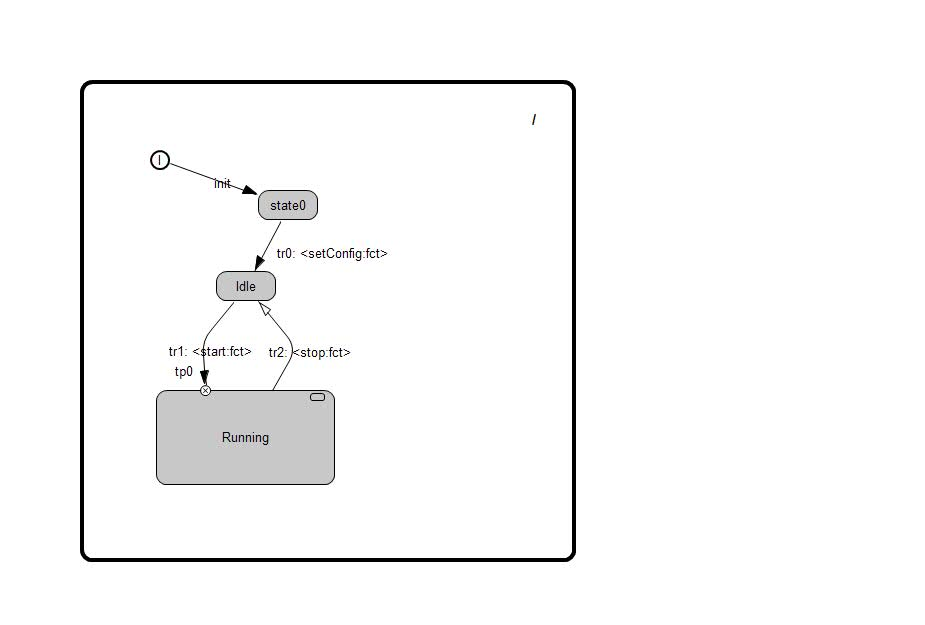
\includegraphics[width=\textwidth]{images/300-Pump_behavior.jpg}
		
		\vspace{\baselineskip}
		\vspace{\baselineskip}
		\vspace{\baselineskip}
		
		\subsubsection{\huge SubSystemClass}
			\hypertarget{ref:SubSystemClass}{}
			
			\textbf{Description:} The SubSystem is main Actor of an executable part of the system. It instantiates the Actor instance tree instance of the application ...
				
				Actor instance tree example:
			
			
			\begingroup
			%\setlength{\tabcolsep}{10pt} % Default value: 6pt
			\renewcommand{\arraystretch}{1.8} % Default value: 1
			\begin{longtable}{p{2.5cm}|p{4cm} p{.5\textwidth}}
				\multicolumn{2}{l}{\textbf{\large Features}} & \\
				\hline
			\multirow{5}{*}{Contains:} & \tabitem \hyperlink{ref:ActorRef}{ActorRef}  & An ActorRef ...description\\
			& \tabitem \hyperlink{ref:RelayPort}{RelayPort}  & RelayPort description \\
			& \tabitem \hyperlink{ref:SPP}{SPP}  & An SPP ... description \\
			& \tabitem \hyperlink{ref:Binding}{Binding}  & A Binding connects two Ports with each otherdescription \\
			& \tabitem \hyperlink{ref:LayerConnection}{LayerConnection}  & A LayerConnection ... description  \\
			\hline
			\end{longtable}
			\endgroup
			
			\begingroup
			%\setlength{\tabcolsep}{10pt} % Default value: 6pt
			\renewcommand{\arraystretch}{1.8} % Default value: 1
			\begin{longtable}{p{2.5cm}|p{4cm} p{.5\textwidth}}
				\multicolumn{2}{l}{\textbf{\large Related Features}} & \\
				\hline
			Typecasts: & \tabitem \hyperlink{ref:SubSystemRef}{SubSystemRef}  & \\
			\hline
			Is contained in: & \tabitem \hyperlink{ref:LogicalModel}{LogicalModel}  & The LogicalModel describes the logical structure and behavior of a ROOM application. The LogicalModel an its elements can be mapped on any PhysicalModel and its elements...\\
			\hline
			\end{longtable}
			\endgroup
			
			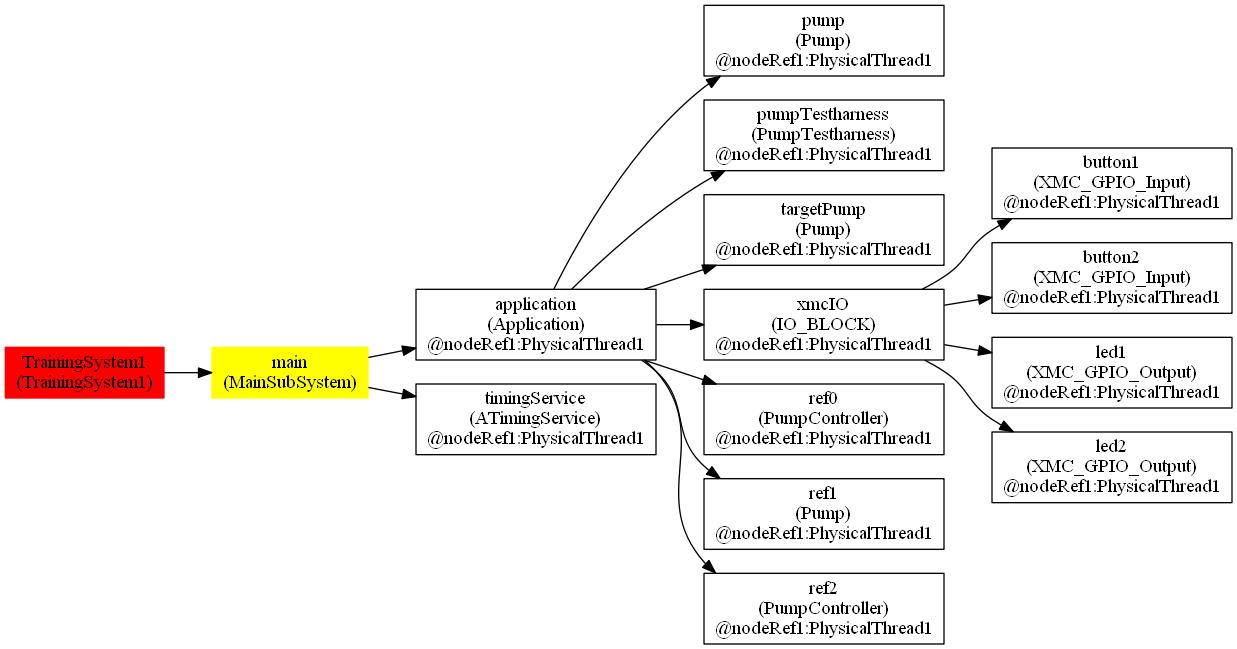
\includegraphics[width=\textwidth]{images/300-TrainingSystem1_instanceTree.jpg}
			
			
		\vspace{\baselineskip}
		\vspace{\baselineskip}
		\vspace{\baselineskip}
		\subsection{\huge PhysicalModel}
		The PhysicalModel describes the topology of the targets a distributed system can be deployed (mapped) on.
	
		
		\subsection{\huge MappingModel}
		The MappingModel describes the mapping of elements of the LogicalModel to elements of the PhysicalModel. It enables the complete decoupling of the LogicalModel and the PhysicalModel, thus providing a maximum flexibility and reuse for the models.
	
		
		\subsection{\huge ConfigModel}
		The ConfigModel describes the Attribute configuration of ActorInstances and PortInstances. 
	
		
\section{\huge ModelEditors}
	
		\subsection{\huge TextualROOMEditor}
		Textual model editor
	
		
		\subsection{\huge GraphicalStructureEditor}
		The Structure Editor allows to edit the Actor Structure in a convenient way. It is possible to create and arrange actor references and ports and to create bindings and layer connections.
	
		
		
		\subsubsection{\huge ActorRefPropertyDialog}
			\hypertarget{ref:ActorRefPropertyDialog}{}
			
			\textbf{Description:} A Dialog to edit structural reference of an ActorRef.
			
			
			\begingroup
			%\setlength{\tabcolsep}{10pt} % Default value: 6pt
			\renewcommand{\arraystretch}{1.8} % Default value: 1
			\begin{longtable}{p{2.5cm}|p{4cm} p{.5\textwidth}}
				\multicolumn{2}{l}{\textbf{\large Features}} & \\
				\hline
			Edits: & \tabitem \hyperlink{ref:ActorRef}{ActorRef}  & An ActorRef ...description\\
			\hline
			\end{longtable}
			\endgroup
			
			\begingroup
			%\setlength{\tabcolsep}{10pt} % Default value: 6pt
			\renewcommand{\arraystretch}{1.8} % Default value: 1
			\begin{longtable}{p{2.5cm}|p{4cm} p{.5\textwidth}}
				\multicolumn{2}{l}{\textbf{\large Related Features}} & \\
				\hline
			Is contained in: & \tabitem \hyperlink{ref:GraphicalStructureEditor}{GraphicalStructureEditor}  & The Structure Editor allows to edit the Actor Structure in a convenient way. It is possible to create and arrange actor references and ports and to create bindings and layer connections.\\
			\hline
			\end{longtable}
			\endgroup
			
			
			
		\vspace{\baselineskip}
		\vspace{\baselineskip}
		\vspace{\baselineskip}
		
		\subsubsection{\huge PortPropertyDialog}
			\hypertarget{ref:PortPropertyDialog}{}
			
			\textbf{Description:} 
			
			
			\begingroup
			%\setlength{\tabcolsep}{10pt} % Default value: 6pt
			\renewcommand{\arraystretch}{1.8} % Default value: 1
			\begin{longtable}{p{2.5cm}|p{4cm} p{.5\textwidth}}
				\multicolumn{2}{l}{\textbf{\large Features}} & \\
				\hline
			Edits: & \tabitem \hyperlink{ref:Port}{Port}  & A Port is an instance of a ProtocolClass and the only interface for an ActorClass. It provides strong decoupling of ActorClasses from each other, thus enabling easy testability, reusability and deployment of Actors to different threads or nodes.description \\
			\hline
			\end{longtable}
			\endgroup
			
			\begingroup
			%\setlength{\tabcolsep}{10pt} % Default value: 6pt
			\renewcommand{\arraystretch}{1.8} % Default value: 1
			\begin{longtable}{p{2.5cm}|p{4cm} p{.5\textwidth}}
				\multicolumn{2}{l}{\textbf{\large Related Features}} & \\
				\hline
			Is contained in: & \tabitem \hyperlink{ref:GraphicalStructureEditor}{GraphicalStructureEditor}  & The Structure Editor allows to edit the Actor Structure in a convenient way. It is possible to create and arrange actor references and ports and to create bindings and layer connections.\\
			\hline
			\end{longtable}
			\endgroup
			
			
			
		\vspace{\baselineskip}
		\vspace{\baselineskip}
		\vspace{\baselineskip}
		
		\subsubsection{\huge SPPPropertyDialog}
			\hypertarget{ref:SPPPropertyDialog}{}
			
			\textbf{Description:} 
			
			
			\begingroup
			%\setlength{\tabcolsep}{10pt} % Default value: 6pt
			\renewcommand{\arraystretch}{1.8} % Default value: 1
			\begin{longtable}{p{2.5cm}|p{4cm} p{.5\textwidth}}
				\multicolumn{2}{l}{\textbf{\large Features}} & \\
				\hline
			Edits: & \tabitem \hyperlink{ref:SPP}{SPP}  & An SPP ... description\\
			\hline
			\end{longtable}
			\endgroup
			
			\begingroup
			%\setlength{\tabcolsep}{10pt} % Default value: 6pt
			\renewcommand{\arraystretch}{1.8} % Default value: 1
			\begin{longtable}{p{2.5cm}|p{4cm} p{.5\textwidth}}
				\multicolumn{2}{l}{\textbf{\large Related Features}} & \\
				\hline
			Is contained in: & \tabitem \hyperlink{ref:GraphicalStructureEditor}{GraphicalStructureEditor}  & The Structure Editor allows to edit the Actor Structure in a convenient way. It is possible to create and arrange actor references and ports and to create bindings and layer connections.\\
			\hline
			\end{longtable}
			\endgroup
			
			
			
		\vspace{\baselineskip}
		\vspace{\baselineskip}
		\vspace{\baselineskip}
		
		\subsubsection{\huge StructureEditiorPalette}
			\hypertarget{ref:StructureEditiorPalette}{}
			
			\textbf{Description:} creates all Kinds of ...  picture with explanation
			
			
			
			\begingroup
			%\setlength{\tabcolsep}{10pt} % Default value: 6pt
			\renewcommand{\arraystretch}{1.8} % Default value: 1
			\begin{longtable}{p{2.5cm}|p{4cm} p{.5\textwidth}}
				\multicolumn{2}{l}{\textbf{\large Related Features}} & \\
				\hline
			Is contained in: & \tabitem \hyperlink{ref:GraphicalStructureEditor}{GraphicalStructureEditor}  & The Structure Editor allows to edit the Actor Structure in a convenient way. It is possible to create and arrange actor references and ports and to create bindings and layer connections.\\
			\hline
			\end{longtable}
			\endgroup
			
			
			
		\vspace{\baselineskip}
		\vspace{\baselineskip}
		\vspace{\baselineskip}
		\subsection{\huge GraphicalBehaviorEditor}
		ModelEditor
	
		
\section{\huge CodeGenerators}
	
		\subsection{\huge CCodeGenerator}
	
		
		\subsection{\huge JavaCodeGenerator}
	
		

